\documentclass[11pt]{article}

\usepackage{graphicx}
\usepackage[margin=1in]{geometry}
\usepackage{fancyhdr}
\usepackage[brazilian]{babel}
\usepackage[utf8]{inputenc}
\usepackage[T1]{fontenc}
\usepackage{url}
\usepackage{cite}
\usepackage{indentfirst}
\usepackage{ragged2e}
\usepackage{float}

\setlength\RaggedRightParindent{15pt}

\setlength\parindent{24pt}
\setlength{\parskip}{5pt plus 1pt}
\setlength{\headheight}{13.6pt}

\newcommand\question[2]{\vspace{.25in}\hrule\textbf{#1: #2}\vspace{.5em}\hrule\vspace{.10in}}
\newcommand\funcionamentortc{\vspace{.10in}\textbf{Explique o funcionamento interno de um RTC. (como ele conta os dias/meses e anos ? gastando pouca energia).}}
\newcommand\consumortc{\vspace{.10in}\textbf{Qual o consumo de energia do RTC no SAME70 ?}}
\renewcommand\part[1]{\vspace{.10in}\textbf{(#1)}}
\pagestyle{fancyplain}
\lhead{\textbf{\NAME\ }}
\chead{\textbf{11 - Tick! Tack!}}
\rhead{\today}


\begin{document}\raggedright
%Section A==============Change the values below to match your information==================
\newcommand\NAME{Marcelo G de Andrade}  % your name
\newcommand\HWNUM{1}              % the homework number
%Section B==============Put your answers to the questions below here=======================

% no need to restate the problem --- the graders know which problem is which,
% but replacing "The First Problem" with a short phrase will help you remember
% which problem this is when you read over your homeworks to study.

\raggedright
\question{1}{Diagrama detalhado}

\begin{figure}[h!]
	\centering
	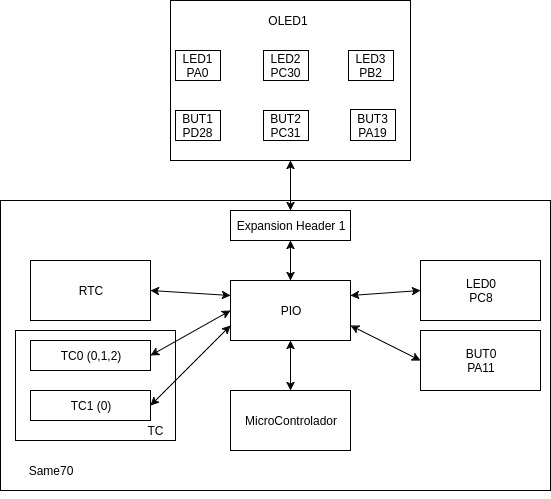
\includegraphics[width=0.7\textwidth]{tictack.jpg}
	\caption{Diagrama de blocos representativo do código da Aula 11.}
\end{figure}


\raggedright
\question{2}{Pesquisa}

\part{1} \funcionamentortc

\RaggedRight
Como é explicado em \cite{rtc}, o RTC(Real Time Clock) é basicamente um relógio que armazena o horário atual. O RTC apresenta uma pequena bateria que mantém seu funcionamento mesmo que o periférico seja desligado. Para contar o tempo, o periférico usa um cristal oscilador ou até a frequência da linha de energia.

\part{4} \consumortc

\RaggedRight
Segundo o datasheet da SAME70, há um consumo de aproximadamente 1.1 \(\mu\)A em modo Backup. Esse consumo considera os periféricos RTC, RTT e a lógica de wake-up ativados.


\bibliography{ref}{}
\bibliographystyle{plain}
\end{document}